\documentclass[a4paper,11pt,         % A4纸
               % twoside,              % 双面
%              openany               % 新章节在偶数页开始
               ]{article}

\usepackage{xeCJK}

%%%%%%%%%% 版面控制 %%%%%%%%%%
\usepackage{indentfirst}             % 首行缩进
\iffalse
\usepackage[%paperwidth=18.4cm, paperheight= 26cm,
            body={14.6true cm,22true cm},
            twosideshift=0 pt,
            %headheight=1.0true cm
            ]{geometry}
\fi
\usepackage[perpage,symbol]{footmisc}% 脚注控制
\usepackage[sf]{titlesec}            % 控制标题
\usepackage{titletoc}                % 控制目录
\usepackage{fancyhdr}                % 页眉页脚
\usepackage{type1cm}                 % 控制字体大小
\usepackage{indentfirst}             % 首行缩进
\usepackage{makeidx}                 % 建立索引
\usepackage{textcomp}                % 千分号等特殊符号
\usepackage{layouts}                 % 打印当前页面格式
\usepackage{bbding}                  % 一些特殊符号
\usepackage{cite}                    % 支持引用
\usepackage{color,xcolor}            % 支持彩色文本、底色、文本框等
\usepackage{listings}                % 粘贴源代码
\usepackage{bm}
\lstloadlanguages{}                  % 所要粘贴代码的编程语言
\lstset{language=,tabsize=4, keepspaces=true,
    xleftmargin=2em,xrightmargin=2em, aboveskip=1em,
    backgroundcolor=\color{lightgray},    % 定义背景颜色
    frame=none,                      % 表示不要边框
    keywordstyle=\color{blue}\bfseries,
    breakindent=22pt,
    numbers=left,stepnumber=1,numberstyle=\tiny,
    basicstyle=\footnotesize,
    showspaces=false,
    flexiblecolumns=true,
    breaklines=true, breakautoindent=true,breakindent=4em,
    escapeinside={/*@}{@*/}
}

%%%%%%%%%%% 代码 %%%%%%%%%%%%%%%%

\usepackage{listings}
\usepackage{xcolor}
% 定义可能使用到的颜色
\definecolor{mygreen}{rgb}{0,0.6,0}
\definecolor{mygray}{rgb}{0.5,0.5,0.5}
\definecolor{mymauve}{rgb}{0.58,0,0.82}

\lstset{ %
  backgroundcolor=\color{white},   % choose the background color; you must add \usepackage{color} or \usepackage{xcolor}
  basicstyle=\footnotesize,        % the size of the fonts that are used for the code
  breakatwhitespace=false,         % sets if automatic breaks should only happen at whitespace
  breaklines=true,                 % sets automatic line breaking
  captionpos=bl,                    % sets the caption-position to bottom
  commentstyle=\color{mygreen},    % comment style
  deletekeywords={...},            % if you want to delete keywords from the given language
  escapeinside={\%*}{*)},          % if you want to add LaTeX within your code
  extendedchars=true,              % lets you use non-ASCII characters; for 8-bits encodings only, does not work with UTF-8
  frame=single,                    % adds a frame around the code
  keepspaces=true,                 % keeps spaces in text, useful for keeping indentation of code (possibly needs columns=flexible)
  keywordstyle=\color{blue},       % keyword style
  %language=Python,                 % the language of the code
  morekeywords={*,...},            % if you want to add more keywords to the set
  numbers=left,                    % where to put the line-numbers; possible values are (none, left, right)
  numbersep=5pt,                   % how far the line-numbers are from the code
  numberstyle=\tiny\color{mygray}, % the style that is used for the line-numbers
  rulecolor=\color{black},         % if not set, the frame-color may be changed on line-breaks within not-black text (e.g. comments (green here))
  showspaces=false,                % show spaces everywhere adding particular underscores; it overrides 'showstringspaces'
  showstringspaces=false,          % underline spaces within strings only
  showtabs=false,                  % show tabs within strings adding particular underscores
  stepnumber=1,                    % the step between two line-numbers. If it's 1, each line will be numbered
  stringstyle=\color{orange},     % string literal style
  tabsize=2,                       % sets default tabsize to 2 spaces
  %title=myPython.py                   % show the filename of files included with \lstinputlisting; also try caption instead of title
}



% 1级标题居中显示
%\titleformat*{\section}{\centering}

%%%%%%%%%% 编号 %%%%%%%%%%%%
\usepackage{enumerate}

%%%%%%%%%% 字体支持 %%%%%%%%%%%%
%\usepackage{ccmap}                  % 使pdfLatex生成的文件支持复制等
\usepackage{CJK,CJKnumb,CJKulem}     % 中文支持
\usepackage{times}     % 包括 Times Roman + Helvetica + Courier
%\usepackage{palatino} % 包括 Palatino + Helvetica + Courier
%\usepackage{newcent}  % 包括 New Century Schoolbook + Avant Garde + Courier
%\usepackage{bookman}  % 包括 Bookman + Avant Garde + Courier

%%%%%%%%%% 代码 %%%%%%%%%%
% \usepackage[ruled, vlined, linesnumbered]{algorithm2e}
\usepackage{algorithm}
\usepackage{algorithmicx}
\usepackage{algpseudocode}

%%%%%%%%%% 数学符号公式 %%%%%%%%%%
\usepackage{latexsym}
\usepackage{amsmath}                 % AMS LaTeX宏包
\usepackage{amssymb}                 % 用来排版漂亮的数学公式
\usepackage{amsbsy}
\usepackage{amsthm}
\usepackage{amsfonts}
\usepackage{mathrsfs}                % 英文花体字体
\usepackage{bm}                      % 数学公式中的黑斜体
\usepackage{relsize}                 % 调整公式字体大小:\mathsmaller, \mathlarger
\usepackage{caption2}                % 浮动图形和表格标题样式

%%%%%%%%%% 图形支持宏包 %%%%%%%%%%
\usepackage{graphicx}
% \ifx\pdfoutput\undefined             % 用latex或pdflatex编译
%   \usepackage[dvips]{graphicx}       % 将eps格式的图片放在figures目录下
% \else                                % 在setup/format.tex中用以下命令注明路径:
%   \usepackage[pdftex]{graphicx}      % \graphicspath{{figures/}}
% \fi
%\usepackage{subfigure}
\usepackage{epsfig}                  % 支持eps图像
%\usepackage{picinpar}               % 图表和文字混排宏包
%\usepackage[verbose]{wrapfig}       % 图表和文字混排宏包
%\usepackage{eso-pic}                % 向文档的部分页加n副图形, 可实现水印效果
%\usepackage{eepic}                  % 扩展的绘图支持
%\usepackage{curves}                 % 绘制复杂曲线
%\usepackage{texdraw}                % 增强的绘图工具
%\usepackage{treedoc}                % 树形图绘制
%\usepackage{pictex}                 % 可以画任意的图形\usepackage{amsbsy}
\usepackage{amsthm}
\usepackage{amsfonts}
\usepackage{mathrsfs}                % 英文花体字体
\usepackage{bm}                      % 数学公式中的黑斜体
\usepackage{relsize}                 % 调整公式字体大小:\mathsmaller, \mathlarger
\usepackage{caption2}                % 浮动图形和表格标题样式

%%%%%%%%%% 表格支持宏包 %%%%%%%%%%
\usepackage{multirow}

%%%%%%%%%% 图形支持宏包 %%%%%%%%%%
\usepackage{graphicx}
% \ifx\pdfoutput\undefined             % 用latex或pdflatex编译
%   \usepackage[dvips]{graphicx}       % 将eps格式的图片放在figures目录下
% \else                                % 在setup/format.tex中用以下命令注明路径:
%   \usepackage[pdftex]{graphicx}      % \graphicspath{{figures/}}
% \fi
%\usepackage{subfigure}
\usepackage{epsfig}                  % 支持eps图像
%\usepackage{picinpar}               % 图表和文字混排宏包
%\usepackage[verbose]{wrapfig}       % 图表和文字混排宏包
%\usepackage{eso-pic}                % 向文档的部分页加n副图形, 可实现水印效果
%\usepackage{eepic}                  % 扩展的绘图支持
%\usepackage{curves}                 % 绘制复杂曲线
%\usepackage{texdraw}                % 增强的绘图工具
%\usepackage{treedoc}                % 树形图绘制
%\usepackage{pictex}                 % 可以画任意的图形
%\usepackage{hyperref}

%%%%%%%%%% 一些距离设置 %%%%%%%%%%%
\setlength{\floatsep}{10pt plus 3pt minus 2pt}       % 图形之间或图形与正文之间的距离
\setlength{\abovecaptionskip}{2pt plus 1pt minus 1pt}% 图形中的图与标题之间的距离
\setlength{\belowcaptionskip}{3pt plus 1pt minus 2pt}% 表格中的表与标题之间的距

%%%%%%%%%% 纸张和页面的大小 %%%%%%%%%%
%\paperwidth   20 true cm            % 纸张宽
%\paperheight  30 true cm            % 纸张高
%\textwidth    10 true cm            % 正文宽
%\textheight   20 true cm            % 正文高
%\headheight      14pt               % 页眉高
%\headsep         16pt               % 页眉距离
%\footskip        27pt               % 页脚距离
%\marginparsep    10pt               % 边注区距离
%\marginparwidth  100pt              % 边注区宽
\makeindex                           % 生成索引
% \pagestyle{fancy}                    % 页眉页脚风格
\fancyhf{}                           % 清空当前页眉页脚的默认设置

%%%%%%%%%% 伪代码 %%%%%%%%%%%
% \floatname{algorithm}{算法}
% \renewcommand{\algorithmicrequire}{\textbf{输入:}}
% \renewcommand{\algorithmicensure}{\textbf{输出:}}

%%%%%%%%%% 导入中文环境 %%%%%%%%%%
% \AtBeginDocument{\begin{CJK*}{GBK}{song} % 不计中文的空格
% \CJKindent                           % 首行缩进两个汉字
% \sloppy\CJKspace                     % 中英文混排的断行
% \CJKtilde                            % 重新定义~,用~隔开中英文
% \CJKcaption{GB}                      % 章节标题的中文化
% }
% \AtEndDocument{\end{CJK*}}

%%%%%%%%%% 正文 %%%%%%%%%%
\begin{document}

%%%%%%%%%% 一些新定义 %%%%%%%%%%
\newcommand{\song}{\CJKfamily{song}} % 宋体
\newcommand{\hei}{\CJKfamily{hei}}   % 黑体
\newcommand{\fs}{\CJKfamily{fs}}     % 仿宋
\newcommand{\kai}{\CJKfamily{kai}}   % 楷体

%%%%%%%%%% 定理类环境的定义 %%%%%%%%%%
%% 必须在导入中文环境之后
\newtheorem{example}{例}             % 整体编号
% \newtheorem{algorithm}{算法}
\newtheorem{theorem}{定理}[section]  % 按 section 编号
\newtheorem{definition}{定义}
\newtheorem{axiom}{公理}
\newtheorem{property}{性质}
\newtheorem{proposition}{命题}
\newtheorem{lemma}{引理}
\newtheorem{corollary}{推论}
\newtheorem{remark}{注解}
\newtheorem{condition}{条件}
\newtheorem{conclusion}{结论}
\newtheorem{assumption}{假设}

%%%%%%%%%% 一些重定义 %%%%%%%%%%
%% 必须在导入中文环境之后
\renewcommand{\contentsname}{目录}     % 将Contents改为目录
\renewcommand{\abstractname}{摘\ \ 要} % 将Abstract改为摘要
\renewcommand{\refname}{参考文献}      % 将References改为参考文献
\renewcommand{\indexname}{索引}
\renewcommand{\figurename}{图}
\renewcommand{\tablename}{表}
\renewcommand{\appendixname}{附录}
\renewcommand{\proofname}{\hei 证明}
% \renewcommand{\algorithm}{\hei 算法}

%%%%%%%%%% 重定义字号命令 %%%%%%%%%%
\newcommand{\yihao}{\fontsize{26pt}{36pt}\selectfont}       % 一号, 1.4倍行距
\newcommand{\erhao}{\fontsize{22pt}{28pt}\selectfont}       % 二号, 1.25倍行距
\newcommand{\xiaoer}{\fontsize{18pt}{18pt}\selectfont}      % 小二, 单倍行距
\newcommand{\sanhao}{\fontsize{16pt}{24pt}\selectfont}      % 三号, 1.5倍行距
\newcommand{\xiaosan}{\fontsize{15pt}{22pt}\selectfont}     % 小三, 1.5倍行距
\newcommand{\sihao}{\fontsize{14pt}{21pt}\selectfont}       % 四号, 1.5倍行距
\newcommand{\bansi}{\fontsize{13pt}{19.5pt}\selectfont}     % 半四, 1.5倍行距
\newcommand{\xiaosi}{\fontsize{12pt}{18pt}\selectfont}      % 小四, 1.5倍行距
\newcommand{\dawu}{\fontsize{11pt}{11pt}\selectfont}        % 大五, 单倍行距
\newcommand{\wuhao}{\fontsize{10.5pt}{10.5pt}\selectfont}   % 五号, 单倍行距

%%%%%%%%%% 表格 %%%%%%%%%%
\newcommand{\tabincell}[2]{\begin{tabular}{@{}#1@{}}#2\end{tabular}}

%%%%%%%%%% 页眉和页脚的设置 %%%%%%%%%%
\lhead{一个~\LaTeX+CJK~的简单模板}
\rhead{\TeX~爱好者}
\lfoot{用~\LaTeX~写科技论文}
\rfoot{~\thepage~}

%%%%%%%%%% 论文标题、作者等 %%%%%%%%%%
\title{Ensembles of Trees 算法与实现}
%\author{BDA小组\\                     % 作者
%        中国科学院计算技术研究所}
\date{January 12, 2015}                % 日期
\maketitle                           % 生成标题
% \tableofcontents                     % 插入目录
% \thispagestyle{empty}                % 首页无页眉页脚





%%%%%%%%%% section %%%%%%%%%%
\section{Regression Trees}

\subsection{算法基础}

回归树(Regression Trees)是一种贪心算法:它将特征空间进行递归地划分,切割成若干块区域,当对预测集的样本点进行预测时,先根据样本特征判断该样本点位于哪块区域,然后用该区域内的训练样本点集的均值作为该样本点的预测集。如图~(\ref{fig:regression_trees_cut})所示。

\begin{figure}[htbp]
\centering\includegraphics[width=3.5in]{img/regression_trees_cut.eps}
\caption{回归树算法}\label{fig:regression_trees_cut}
\end{figure}

\subsubsection{构造过程}

回归树的构造采用的是二分递归分割的方法,从根节点开始“生长”。在每个节点处(初始只有一个根节点),选取某维特征的某个特征值作为分裂阈值,将当前节点所包含的样本集分成两个子样本集(根节点包含所有的训练样本),形成两个子节点,再对子节点采用同样的方法继续分割,直到不满足分割条件为止。如图~(\ref{fig:regression_trees})所示。 \\

因此,回归树是结构简单的二叉树。 

\begin{figure}[htbp]
\centering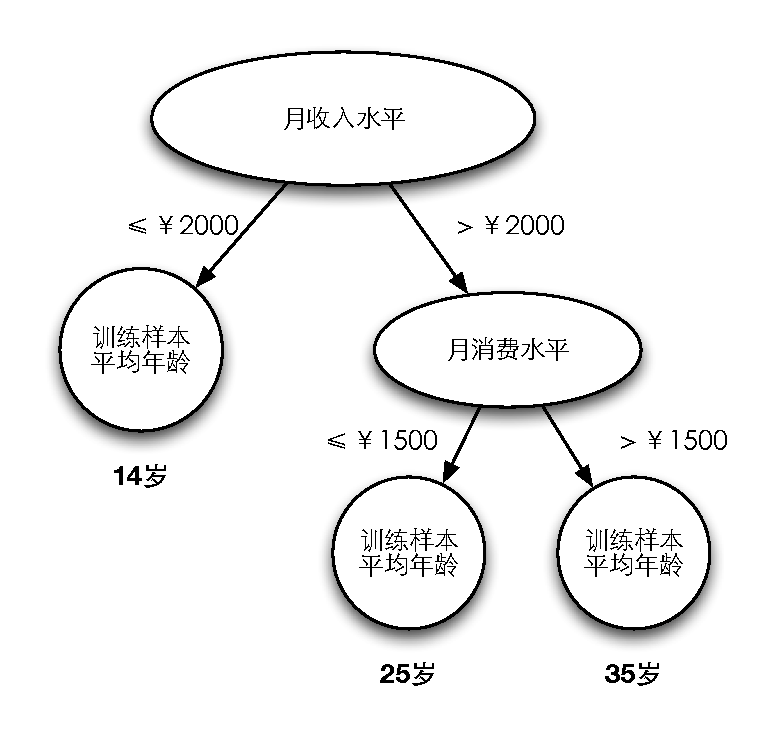
\includegraphics[width=3.5in]{img/regression_trees.eps}
\caption{回归树构造过程}\label{fig:regression_trees}
\end{figure}

\subsubsection{节点纯度}

%在回归树构造的过程中,会根据一定的标准分裂节点。在本算法中,每个节点分裂所使用的特征及对应特征值的选取依据的是方差(Variance)

在回归树的构造过程中,每次节点的分裂都会生成两个新的节点,我们使用节点上所对应的训练样本集合的方差(Variance)来衡量该节点的优劣程度(不纯度, Impurity)。方差越大,则对应节点越混乱,质量越差。节点$N$的方差的计算方法如公式~(\ref{eqt:variance})所示。

\begin{eqnarray}
	\label{eqt:variance}
{I}_{v}(N)=\frac{1}{{\left|S \right|}^{2}}\sum_{i\in S}\sum_{j\in S}\frac{1}{2}(y_{i}-y_{j})^2
\end{eqnarray}

其中,$S$表示节点$N$所包含的训练样本集,$y_{i}$表示节点$N$所包含的训练样本集中的第$i$个样本点的$label$值。 \\

在实现的过程中,为了提高算法的效率,采用了公式~(\ref{eqt:variance})的另一种表示形式,如公式~(\ref{eqt:variance2})所示。

\begin{eqnarray}
	\label{eqt:variance2}
{I}_{v}(N)=\frac{1}{\left | S \right |}\left ( \sum_{i\in S} {y_{i}}^2 - \frac{1}{\left | S \right |} \sum_{i \in S} {y_{i}}^2 \right )
\end{eqnarray}

\subsubsection{信息增益}

每个节点在分裂的时候有多种分裂方式可供选择,最终选取何种分裂方式依据的是该分裂方式所带来的信息增益(Information Gain)。在回归树中,使用节点分裂的方差缩减量(Variance Reduction)来表示本次分裂的信息增益,方差缩减量越大,说明这次分裂的效果越好。该信息增益的计算方法如公式~(\ref{eqt:variance_reduction})所示。

\begin{eqnarray}
	\label{eqt:variance_reduction}
IG_{v}(N) = I_{v}(N) - \left ( \frac{\left | S_{1}\right |}{\left | S \right |} I_{v}\left ( N_{1} \right ) + \frac{\left | S_{2}\right |}{\left | S \right |} I_{v}\left ( N_{2} \right )\right)
\end{eqnarray}

其中,$N_{1}$、$N_{2}$表示分裂过程中由$N$新生成的两个子节点,$S$表示节点$N$所包含的训练样本集,$S_{1}$表示子节点$N_{1}$所包含的训练样本集,$S_{2}$表示子节点$N_{2}$所包含的训练样本集。

\subsubsection{终止条件}

回归树的节点在遇到如下情况的时候终止分裂,形成叶子节点:

% \begin{enumerate}[(1)]
\begin{itemize}
\item 节点分裂带来的信息增益小于用户指定的最小信息增益($min\_info\_gain$)。
\item 节点树深大于等于用户指定的最大树深($max\_depth$)。
\item 节点权重小于等于用户指定的节点最小权重($min\_node\_size$)。
\end{itemize}
% \end{enumerate}

\subsubsection{叶节点预测值}

每个叶子节点对应一个预测值,该预测值的计算方法如公式~(\ref{eqt:leave_pred})所示。

\begin{eqnarray}
	\label{eqt:leave_pred}
P_{i} = \frac{1}{\left | S_{i} \right |} \sum_{j \in S_{i}} y_{ij}
\end{eqnarray}

其中,~$P_{i}$~表示第$i$个叶子节点的预测值,~$S_{i}$~表示第$i$个叶子节点上的训练样本集,~$y_{ij}$~表示第$i$个叶子节点所包含的训练样本集中的第$j$个样本点的$label$值。

\subsection{分布式实现}

\subsubsection{特征值分箱}

为了使模型能够适应大规模数据的需求,在为节点分裂选择合适的特征及阈值的过程中,算法没有遍历每个特征的所有特征值,而是先对训练样本采样,将采样的训练样本中每个特征的特征值尽可能均匀的分箱(箱中的训练样本个数尽可能相等),使用箱与箱之间的边界值作为候选该特征的候选分裂值。如图~(\ref{fig:feature_bins})所示。

\begin{figure}[htbp]
\centering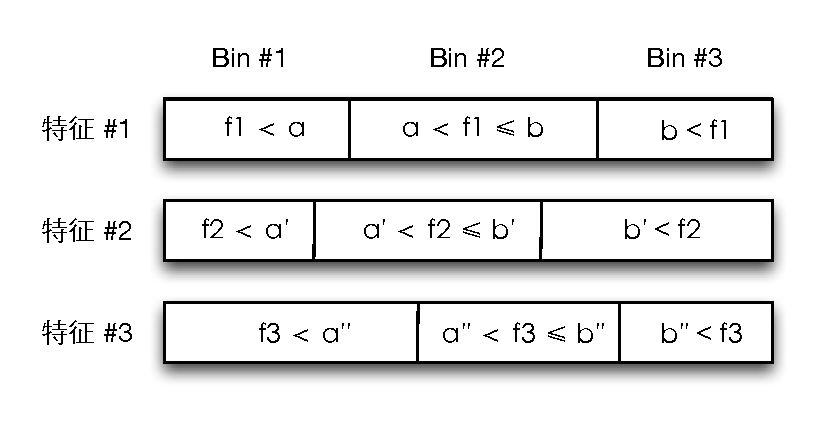
\includegraphics[width=3.5in]{img/feature_bins.eps}
\caption{特征值分箱}\label{fig:feature_bins}
\end{figure}

\subsubsection{最优分裂方式选择}

在回归树的分布式实现中,训练数据集存储在集群的不同机器节点上。为了给每个节点选择一个最优的分裂方式(分裂使用的特征及分裂阈值),集群的每个机器节点为每个待分裂节点维护三个统计量:该机器节点上的训练集分区中属于该待分裂节点的样本个数($count$)、样本$label$之和($sum$)以及样本$label$的平方和($squared\_sum$)。最后,将各机器节点维护的统计量收集到Driver所在的机器节点,在该机器节点上依据这些统计量完成最优分裂方式的选择。如图~(\ref{fig:best_split})所示。

\begin{figure}[htbp]
\centering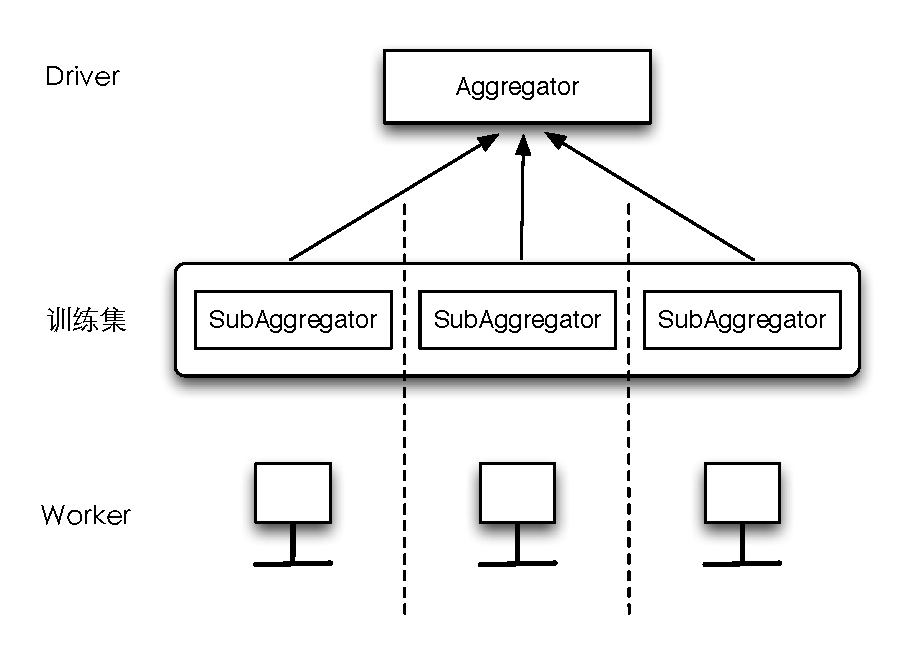
\includegraphics[width=3.5in]{img/best_split.eps}
\caption{最优分裂方式选择}\label{fig:best_split}
\end{figure}

\subsection{使用示例}

\begin{lstlisting}[language={SCALA},title={RunDecisionTreeDemo.scala}]  
// read training data and testing data from disk
val train = Points.readLibSVMFile(sc, data_dir + "cadata.train")
val test = Points.readLibSVMFile(sc, data_dir + "cadata.test")

train.cache()
test.cache()

// train a model of decision tree
val model: DecisionTreeModel = DecisionTree.train(
  train_data = train,
  valid_data = null,
  impurity = "Variance",
  loss = "SquaredLoss",
  max_depth = 10,
  max_bins = 32,
  bin_samples = 10000,
  min_node_size = 15,
  min_info_gain = 1e-6,
  row_rate = 1.0,
  col_rate = 1.0,
  silent = false)

// predict for testing data use the model
val predictions = model.predict(test).zip(test).map {
  case (y, pn) => s"$y\t$pn"
}
// save predictions on disk
predictions.saveAsTextFile(prediction_pt)

// save the model on disk
model.save(sc, model_pt)
\end{lstlisting}  

\section{GBRT}

\subsection{算法基础}

GBRT(Gradient Boosting Regression Trees)是迭代的回归树算法。该算法模型由多棵回归树构成,所有回归树的预测结果的累加值即为最终的预测值。GBRT是一种泛化能力(Generalization)很强的算法。

\subsubsection{回归树}

回归树是GBRT的基本组成单位,用来做回归分析。回归树在上一节进行了详细的说明,此处不再赘述。

% GBRT的每一轮迭代都会生成一棵新的回归树,将所有训练得到的回归树的预测值按一定方式累加作为预测值,与真实值一起代入损失函数并求预测值偏导,得到的数据作为下一轮的输入,继续迭代。 \\

\subsubsection{梯度迭代}

GBRT的每一轮迭代都会生成一棵新的回归树,将所有训练得到的回归树的预测值按一定方式累加作为预测值,与真实值一起代入损失函数并求预测值偏导,得到的数据作为下一轮的输入,继续迭代。 \\

伪代码~(\ref{alg:gb})详细说明了GBRT算法中梯度迭代的执行过程,即如何构建回归树模型并将其进行组合。

\begin{algorithm}
	\caption{Gradient tree boosting for multiple additive regression trees}
	\label{alg:gb}
	\begin{algorithmic}[1] %每行显示行号
	\State $f_{0} \gets argmin_{\gamma} \sum_{i = 1}^{N} L \left ( y_{i}, \gamma\right )$
	\For{$m = 1 \to M$}
		\For{$i = 1 \to N$}
			\State $r_{im} \gets -\left [ \frac{\partial L\left ( y_{i}, f\left ( x_{i} \right ) \right )}{\partial f\left ( x_{i} \right )} \right ]_{f=f_{m-1}}$			
		\EndFor
		\State Fit a regression tree to the targets $r_{im}$ giving terminal regions $R_{jm}, j = 1,2,...,J_{m}$.
		\For{$j = 1 \to J_{m}$}
			\State $\gamma_{jm} \gets argmin_{\gamma} \sum_{x_{i} \in R_{jm}} L\left ( y_{i},f_{m-1}\left ( x_{i} \right ) + \gamma \right )$
		\EndFor
		\State $f_{m}\left ( x \right ) \gets f_{m-1}\left ( x \right ) + \sum_{j=1}^{J_{m}} \gamma_{jm}I\left ( x \in R_{jm} \right )$
		\label{alg:gb:update}
	\EndFor
	\State Output $\hat{f}\left ( x \right ) \gets f_{M}\left ( x \right )$
	\end{algorithmic}
\end{algorithm}

\subsubsection{缩减思想}

缩减(Shrinkage)的思想认为,在模型的迭代过程中,每次走一小步逐渐逼近结果的效果,要比每次都一大步很快逼近结果的方式更容易避免过拟合,同时也更容易收敛。 \\

也就是说,我们不能完全信任每一棵决策树,每一棵决策树只能学到真理的一小部分,累加的时候只累加一小部分,通过多棵决策树来弥补不足。 \\

因此,对伪代码~($\ref{alg:gb}$)~第~($\ref{alg:gb:update}$)~行的公式进行修改,如公式~($\ref{eqt:learning_rate}$)~所示。其中,$\rho_{m}$通常被称作学习率(Learning Rate)。
\begin{eqnarray}
	\label{eqt:learning_rate}
	f_{m}\left ( x \right ) \gets f_{m-1}\left ( x \right ) + \rho_{m} \sum_{j=1}^{J_{m}} \gamma_{jm}I\left ( x \in R_{jm} \right )
\end{eqnarray}

\subsection{使用示例}

\begin{lstlisting}[language={SCALA},title={RunGradientBoostDemo.scala}]  
// read training data and testing data from disk
val train = Points.readLibSVMFile(sc, data_dir + "cadata.train")
val test = Points.readLibSVMFile(sc, data_dir + "cadata.test")

train.cache()
test.cache()

// train a model of decision tree
val model: GradientBoostModel = GradientBoost.train(
  train_data = train,
  valid_data = null,
  impurity = "Variance",
  loss = "SquaredLoss",
  max_depth = 10,
  max_bins = 32,
  min_samples = 10000,
  min_node_size = 15,
  min_info_gain = 1e-6,
  row_rate = 0.6,
  col_rate = 0.6,
  num_iter = 20,
  learn_rate = 0.02,
  min_step = 1e-6, 
  silent = false)

// predict for testing data use the model
val predictions = model.predict(test).zip(test).map {
  case (y, pn) => s"$y\t$pn"
}
// save predictions on disk
predictions.saveAsTextFile(prediction_pt)

// save the model on disk
model.save(sc, model_pt)
\end{lstlisting}  

\section{随机森林}

\subsection{基本思想}

随机森林算法生成很多棵回归树,当对新的样本进行预测的时候,随机森林中的每一棵树都会给出自己的预测值,并由此进行“投票”,在回归问题中,随机森林的输出是所有回归树输出的平均值。

\subsubsection{随机采样}

随机森林模型的构建中,存在两个随机过程:对样本的有放回采样和对特征的无放回采样。

\begin{itemize}
  \item 对样本的有放回采样,用来训练每一棵回归树。
  \item 对特征的无放回采样,用做回归树节点的每一次分裂。
\end{itemize}

\subsubsection{伪代码}

随机森立的执行过程如伪代码~(\ref{alg:rf})所示。


\begin{algorithm}
  \caption{Random forest}
  \label{alg:rf}
  \begin{algorithmic}[1] %每行显示行号
  \For{$m = 1 \to M$}
    \State Sample, with replacement from $\mathbf{X}$, $\mathbf{Y}$; call these $\mathbf{X_{m}}$, $\mathbf{Y_{m}}$.
    \State Fit a regression tree to the targets $y_{im}$($y_{im} \in \mathbf{Y_{m}}$) giving terminal regions $R_{jm}, j = 1,2,...,J_{m}$(Sample features without replacement during nodes splitting of the regression tree).
    \For{$j = 1 \to J_{m}$}
      \State $\gamma_{jm} \gets argmin_{\gamma} \sum_{x_{i} \in R_{jm}} L\left ( y_{i},f_{m-1}\left ( x_{i} \right ) + \gamma \right )$
    \EndFor
    \State $f_{m}\left ( x \right ) \gets f_{m-1}\left ( x \right ) + \sum_{j=1}^{J_{m}} \gamma_{jm}I\left ( x \in R_{jm} \right )$
  \EndFor
  \State Output $\hat{f}\left ( x \right ) \gets  \frac{1}{M} f_{M}\left ( x \right )$
  \end{algorithmic}
\end{algorithm}

\subsection{使用示例}

\begin{lstlisting}[language={SCALA},title={RunRandomForestDemo.scala}]  
// read training data and testing data from disk
val train = Points.readLibSVMFile(sc, data_dir + "cadata.train")
val test = Points.readLibSVMFile(sc, data_dir + "cadata.test")

train.cache()
test.cache()

// train a model of decision tree
val model: RandomForestModel = RandomForest.train(
  train_data = train,
  valid_data = null,
  impurity = "Variance",
  loss = "SquaredLoss",
  max_depth = 10,
  max_bins = 32,
  min_samples = 10000,
  min_node_size = 15,
  min_info_gain = 1e-6,
  row_rate = 0.6,
  col_rate = 0.2,
  num_trees = 20,
  silent = false)

// predict for testing data use the model
val predictions = model.predict(test).zip(test).map {
  case (y, pn) => s"$y\t$pn"
}
// save predictions on disk
predictions.saveAsTextFile(prediction_pt)

// save the model on disk
model.save(sc, model_pt)
\end{lstlisting} 


% \TeX~有诸如AMS\TeX、\LaTeX~等宏库。在~FreeBSD~下,缺省的宏库是~te\TeX。
% Knuth~用~\$~符号界定数学公式,意味着每个好的公式都是无价之宝。
% 有了~\TeX~系统,输入数学公式变得简单愉快。如,
% \begin{theorem}[L\'{e}vy\index{L\'{e}vy~定理}]
% 令~$F(x),\varphi(t)$~分别为随机变量~$X$~的分布函数和特征函数。
% 假定~$F(x)$~在~$a+h$~和~$a-h (h>0)$~处连续,则有
% \begin{eqnarray}
%   \label{Levy theorem}  % 方程的标记可以是专有名词
% F(a+h)-F(a-h)&=&\lim_{T\rightarrow\infty} \frac{1}{\pi}\int^{T}_{-T} \frac{\sin ht}{t} e^{-ita} \varphi(t)dt
% \end{eqnarray}
% \end{theorem}
% \begin{proof}
%   从略。感兴趣的读者可以参考……。
% \end{proof}
% L\'{e}vy~定理在分布函数和特征函数之间搭建了一座桥梁。由公式~(\ref{Levy theorem})~可得
% \begin{eqnarray}
%   \label{DensityCharacteristic}   % 自定义的标记
%   f(x)&=&\frac{1}{2\pi}\int^{+\infty}_{-\infty} e^{-itx}\varphi(t)dt
% \end{eqnarray}

% \begin{eqnarray}
%   \frac{F(x+\Delta x)-F(x)}{\Delta x}&=&\frac{1}{2\pi} \int^{+\infty}_{-\infty}
% \frac{\sin(t\Delta x/2)}{t\Delta x/2} e^{-it(x+\Delta x/2)} \varphi(t) dt\nonumber\\
%   f(x)&=&\frac{1}{2\pi} \int^{+\infty}_{-\infty} \lim_{\Delta x\rightarrow 0}
% \frac{\sin(t\Delta x/2)}{t\Delta x/2} e^{-it(x+\Delta x/2)} \varphi(t) dt\nonumber\\
%   &=&\frac{1}{2\pi}\int^{+\infty}_{-\infty} e^{-itx}\varphi(t)dt\nonumber
% \end{eqnarray}
% 我们知道特征函数的定义是
% \begin{eqnarray}
%   \label{section1:characteristic}   % 标记中注明了章节号
%   \varphi(t)&=& E(e^{itX})\nonumber\\
%             &=& \int^{+\infty}_{-\infty} e^{itx} f(x)dx
% \end{eqnarray}
% 对比~(\ref{DensityCharacteristic})~和~(\ref{section1:characteristic})~可见,
% 密度函数和特征函数之间的关系非常巧妙。
% % \end{proof}
% \HandRight 在~\TeX~环境里,数学公式的表达是很自然的,绝大多数命令就是英文的数学
% 专有名词或它们的缩写,如果你以前读过英文的数学文献,记忆这些命令是不难的。
% 手头有个命令快速寻查表是很方便的,
% 我用的是~Hypertext Help with \LaTeX,网上可以搜到,是免费的。

% %%%%%%%%%% section %%%%%%%%%%
% \section{符号、字体、颜色等}
% \begin{itemize}
%   \item 特殊字符:\# \$ \% \^{} \& \_ \{ \} \~{} $\backslash \cdots$
%   \item 中文字体:{\song 宋体} {\kai 楷体} {\hei 黑体} {\fs 仿宋}
%   \item 字体大小:{\tiny tiny} {\small small} {\normalsize normalsize}
%                   {\large large} {\Large Large} {\huge huge} {\Huge Huge}
%   \item 汉字大小:{\wuhao 五号} {\dawu 大五} {\xiaosi 小四} {\sihao 四号}
%                   {\xiaosan 小三} {\sanhao 三号} {\xiaoer 小二} {\erhao 二号} {\yihao 一号}
%   \item 各种颜色:{\color{red} 红色} {\color{yellow} 黄色} {\color{blue} 蓝色}
%                   {\color{magenta} 洋红} {\color{cyan} 蓝绿}
% \end{itemize}
% %%%%%%%%%%% section %%%%%%%%%%
% \section{图形表格等浮动对象}

% \index{贝叶斯方法}贝叶斯方法~\cite{Gelman}~主要用于小样本数据分析,它利用参数先验分布和
% 后验分布之差异进行统计推断,其一般步骤是:
% \begin{enumerate}
%   \item 构建概率模型,包括参数的先验分布。
%   \item 给定观察数据,计算参数的后验分布。
%   \item 分析模型的效果,如有必要,回到第一步。
% \end{enumerate}
% 下面,我们给一个表格的例子:
% \begin{center}
% \begin{table}[!h]     % 强制在原位显示表格
% \centering
% \caption{二维随机向量$(X,Y)$的边缘分布}
% \begin{tabular}{l|ccccc|c}
%   $_X$\hspace{3mm} $^Y$&$y_1$&$y_2$&$\cdots$&$y_j$&$\cdots$\\
% \hline
% $x_1$   &$p_{11}$&$p_{12}$&$\cdots$&$p_{1j}$&$\cdots$&$p_{1\cdot}$\\
% $x_2$   &$p_{21}$&$p_{22}$&$\cdots$&$p_{2j}$&$\cdots$&$p_{2\cdot}$\\
% $\vdots$&$\vdots$&$\vdots$&$\vdots$&$\vdots$&$\vdots$&$\vdots$ \\
% $x_i$   &$p_{i1}$&$p_{i2}$&$\cdots$&$p_{ij}$&$\cdots$&$p_{i\cdot}$\\
% $\vdots$&$\vdots$&$\vdots$&$\vdots$&$\vdots$&$\vdots$&$\vdots$ \\
% \hline
%    &$p_{\cdot 1}$&$p_{\cdot 2}$&$\cdots$&$p_{\cdot j}$&$\cdots$&1
% \label{marginal distribution}
% \end{tabular}
% \end{table}
% \end{center}
% 在表~\ref{marginal distribution}中,$p_{\cdot j}=\sum\limits_i p_{ij}$,类似地,$ p_{i\cdot}=\sum\limits_j p_{ij}$。
% % 插入一个图片
% %\includegraphics[width=50mm,height=40mm]{figures/demo.eps}

% %%%%%%%%%% section %%%%%%%%%%
% \section{生成索引}
% 键入命令:makeindex  文件名。\newline
% \indent 譬如对这个模板,生成~Template4CJK.ind~的过程如下。
% \begin{lstlisting}
% $ makeindex Template4CJK
% This is makeindex, version 2.14 [02-Oct-2002] (kpathsea + Thai support).
% Scanning input file Template4CJK.idx....done (4 entries accepted, 0 rejected).
% Sorting entries....done (9 comparisons).
% Generating output file Template4CJK.ind....done (18 lines written, 0 warnings).
% Output written in Template4CJK.ind.
% Transcript written in Template4CJK.ilg.
% \end{lstlisting}

% \printindex % 打印出索引名及其所在页码,即那些\index{索引名}
% %%%%%%%%%% 参考文献 %%%%%%%%%%
% \begin{thebibliography}{}
% \bibitem[Gelman et~al., 2004]{Gelman} Gelman, A., Carlin, J.~B., Stern, H.~S.  \& Rubin, D.~B. (2004)
% Bayesian Data Analysis (Second Edition).  \newblock Chapman \& Hall/CRC.
% \end{thebibliography}
\clearpage
\end{document}
%%%%%%%%%% 结束 %%%%%%%%%%

